 Chapter 2

\chapter{Time Independent Case - A Starting Point} % Main chapter title

\label{Chapter2} % For referencing the chapter elsewhere, use \ref{Chapter2} 

%----------------------------------------------------------------------------------------

\section{Central Finite Difference Methods}
*Assume overview of FD methods covered in Ch.1*
\subsection{Backwards Terms}
In Chapter 1, we introduced the `1 point forward finite difference' method; an alternative to this approach is to use a `backwards finite difference' method, where instead of approximating 
\begin{equation*}
    \delta f\left(x\right) \simeq \frac{f\left(x + h\right) - f\left(x\right)}{h}
\end{equation*}
we instead approximate it as 
\begin{equation*}
    \delta f\left(x\right) \simeq \frac{f\left(x\right) - f\left(x - h\right)}{h}
\end{equation*}
i.e., approximating each point from the succeeding point rather than preceding. 
These are both accurate to a tolerance of $O(h)$, and provide reasonable approximations in cases where there are no sharp peaks or discontinuities in the function over intervals narrow with respect to $h$, as these features can either be missed or cause $\delta f(x)$ to be poorly approximated in these areas. One way to obtain a more accurate estimate of $\delta f(x)$, and limit the impact of potential peaks / discontinuities is to use a `central finite difference' method;
\begin{equation*}
    \delta f\left(x\right) \simeq \frac{f\left(x + h\right) - f\left(x - h\right)}{2h}.
\end{equation*}
It can be seen easily here that the same number of function calls to $f$ are required here, and so the computational expense is the same as previously, but we obtain an estimate accurate to $O(h^{2})$. Additionally, by using both forward and backward points, we limit the impact of sharp features in the function over the interval.

\subsection{End Points}
We have seen that a CFD method will give us a more accurate approximation to $\delta f(x)$, provided that we know the values of the function at points to either side of the point in question; this leads to the problem that at the end points of our interval, we won't know one of these points. There is no singular solution to this problem, as this CFD approach can be applied to a wide variety of problems. In our case, from physical intuition we know that at distances far away from the particle the wavefunction should be near-zero - using this we can choose to model $f(\alpha)$ for any $\alpha$ outside of our interval as $0$, allowing us to use the CFD even at the end points.

\subsection{Getting Coefficients}
In general, any number of points can be used for a finite difference method; with the expected accuracy of the approximation increasing with each additional point. In these cases, not all points contribute equally to the approximation. The set of ratios at which they contribute are called the `finite difference coefficients' of that finite difference scheme. These coefficients can be calculated by solving a system of linear equations (* CITE *);
\begin{align*}
\begin{pmatrix}
1&1&...&1&1\\
-q&-q+1&...&p-1&p\\
(-q)^{2}&(-q+1)^{2}&...&(p-1)^{2}&p^{2}\\
...&...&...&...&...\\
...&...&...&...&...\\
...&...&...&...&...\\
(-p)^{p+q}&(-p+1)^{p+q}&...&(p-1)^{p+q}&p^{p+q}
\end{pmatrix}{\begin{pmatrix}
a_{-q}\\
a_{-q+1}\\
a_{-q+2}\\
...\\
...\\
...\\
a_{p}
\end{pmatrix}} = {\begin{pmatrix}
0\\
0\\
0\\
...\\
m!\\
...\\
0
\end{pmatrix}}
\end{align*}
Where $p$ refers to the number of backward points being used in the approximation of the point in question and $q$ the number of forward points. For a CFD setup, $p=q$. 
$a_{i}$ is the $i^{\text{th}}$ coefficient, and $m$ the order of the derivative being approximated. Cramer's rule, or another method, can then be used to solve the system of linear equations to obtain $\{a_{i}\}$.

Finite Difference approximations, in cases like ours where function values at points outside the interval of interest are taken to be $0$, can be described in matrix form as an eigenvalue problem; 
\begin{align*}
    \left[\frac{-\hbar^{2}}{2m}\frac{d^2}{dr^2} + V\left(r\right)\right] \Psi\left(r\right) = E\Psi\left(r\right)\\
\end{align*}
can be approximated with a CFD method as
\begin{align*}
    \begin{pmatrix}
        a_{0}+V\left(r_{0}\right)&a_{1}&...&a_{p}&0&...\\
        a_{-1}&a_{0}+V\left(r_{1}\right)&...&...&...&...\\
        ...&...&...&...&...&...\\
        0&...&...&a_{-p}&...&a_{0}+V\left(r_{n}\right)
    \end{pmatrix}\mathbf{\Psi_{i}\left(r\right)}\ =\ E_{i}\mathbf{\Psi_{i}\left(r\right)}.
\end{align*}
where $\{E_{i}\}$ and $\{\mathbf{\Psi_{i}}\}$ are eigenvalues and eigenvectors of the matrix; forming a basis set for all possible solutions. Further, physical significance can be inferred from these values; each eigenvalue corresponds to the energy of a distinct state, and states corresponding to negative energies are `bound' states.

\subsection{Useful Properties of CFD method in matrix form}
\begin{itemize}
\item[-]Sparse: \\ From the above equation it can be seen that other than along the central diagonal, and a few off-central diagonals, all elements in the matrix are $0$; meaning that for a large model (high accuracy), the matrix is very sparse. Krylov Subspace based Arnoldi methods are known to be extremely efficient at finding eigenvectors of sparse matrices, due largely to the fact that they rely on repeated QR decomposition (* CITE SAAD *) which involves conversion to a Hessenberg matrix and then to a triangular matrix - which is much faster to do when the matrix is already almost in Hessenberg form (or already in Hessenberg form in the case of a three point or fewer method).
\item[-]Hermitian: \\ As all of the finite difference coefficients are real, and assuming the arbitrary potential function $V$ is real-valued at all points, the entire matrix is real. Additionally, for any CFD method, the matrix is symmetric. Combining these two statements, we have that the matrix is Hermitian; knowing this we can choose the eigensolver carefully to make use of this, for example using one based on Lanczos iteration - a special case of Arnoldi iteration with stages removed due to knowledge that the matrix is Hermitian.
\end{itemize}

\section{Implementation}
\subsection{General Approach}
\begin{itemize}
	\item[>]{\textbf{Overview - Python tools}\\ \noindent\rule{4.5cm}{0.25pt}}

    \item[>]{Set up a set of equally spaced points spanning an interval containing the particle - numpy.linspace}
    \item[>]{Calculate the potential at each of the points - custom defined function}
    \item[>]{Build a `baseline' Hamiltonian of FD coefficients along the appropriate diagonals and $0$ elsewhere - numpy.zeros}
    \item[>]{Add the potential values to the central diagonal - no extra tool needed}
    \item[>]{Use an eigensolver algorithm / tool to find eigenpairs of the Hamiltonian - numpy.linalg.eig}
\end{itemize}

\subsection{Notes On Finding Eigenpairs}
Most eigensolvers, including all of the ones I use in the course of this investigation, are based on variations on Krylov Subspace Iteration. Krylov Subspace Iteration in turn is a particular case of Subspace Iteration, which is a generalised application of Power Iteration. To provide insight to how the eigensolvers work, and later optimisation techniques, I explain here in detail the Power Iteration method followed by outlines of adaptions to it for Subspace Iteration and how the outcome differs for that, followed by similar outlines for the other methods. 


Power Iteration is a method for obtaining the dominant (largest corresponding eigenvalue) eigenvector, $\mathbf{x}$, of a square matrix, $A$. Approximations to $x$ of increasing accuracy are given recursively by
\begin{align*}
	\mathbf{x_0} = \text{any non-zero random vector of the right length}\\
	\mathbf{x_{n}} = \frac{A\mathbf{x_{n-1}}}{||A\mathbf{x_{n-1}}||}
\end{align*}

We know from (* REF CH1 *) that an arbitrary vector, $v$ in the space described by $A$ can be spectrally decomposed into a weighted sum of eigenvectors, $\{\mathbf{e_{i}}\}$ of $A$; $\mathbf{v} = \sum_{i}{c_{i}\mathbf{e_{i}}} for \{c_{i}\} \in \mathbb{C}$.

Therefore we can write $A\mathbf{v}$ as $A\sum_{i}{c_{i}\mathbf{e_{i}}}$, and by orthogonality of eigenvectors we can rewrite this as $\sum_{i}{c_{i}\left(A\mathbf{e_{i}}\right)}$. 

By the definition of an eigenvector, each $A\mathbf{e_i}$ is equal to $\lambda_{i}\mathbf{e_i}$ where $\lambda_i$ is the eigenvalue of that eigenvector. This allows us to further re-write $A\mathbf{v}$ as $\sum_{i}{c_{i}\left(\lambda_{i}\mathbf{e_{i}}\right)}$. 

From (* REF CH1 *), we additionally have that if $(\lambda,\mathbf{e})$ is an eigenpair of $B$, then $(\lambda^{k},\mathbf{e})$ is an eigenpair of $B^{k}$. Applying this here, we have that $A^{k}\mathbf{v}$ can be written as $\sum_{i}{c_{i}\left(\lambda_{i}^{k}\mathbf{e_{i}}\right)}$. 

From this it is clear that, for a high enough $k$, the term in the summation with the largest eigenvalue will be far larger than any other term - making it a good approximation for the most dominant eigenvalue after renormalisation. 

Additionally it can be seen that the error in this approximation can be estimated using the next-largest eigenvalue; $\epsilon \simeq |\frac{\lambda_1}{\lambda_2}|^{k}$ where $\lambda_1, \lambda_2$ are the two most dominant eigenvalues. This shows that the rate of convergence is given by $|\frac{\lambda_1}{\lambda_2}|$.


Subspace Iteration is an extension to Power Iteration, where a set of $m$ random vectors are initialised instead of onle one, and these are repeatedly multiplied by $A$, then orthonormalised with respect to each other (as opposed to simply normalised like the Power Iteration method). The orthonormalisation process, usually done via repeated QR decomposition, ensures that the initial vectors will not all converge to the same, largest, eigenvector - instead one will converge to the next most dominant one, another to the third most, all the way to the $m^{\text{th}}$ most dominant.


Krylov Subspace Iteration is a special case of Subspace Iteration where the initial subspace is not fully random vectors, and is instead built from a single random vector, $\mathbf{b}$, such that the subspace consists of vectors $\{\mathbf{b}, A\mathbf{b},...,A^{m}\mathbf{b}\}$. One reason to use a Krylov subspace over a randomised one is that vectors in the Krylov subspace will have large spectral components for dominant eigenvectors, as shown in the above proof of Power Iteration convergence. This results in in a reduced number of subspace iterations needed for convergence.


Other improvements on these methods exist, including the `implicitly restarted Arnoldi' method and `Hermitian Lanczos' method - which I do not describe further here, other than to describe the Lanczos method as being able to ignore redundant steps in the case that $A$ is Hermitian.


In this investigation, while I made use of these results through eigensolver choice and parameter tuning, I did not recreate any of these algorithms directly; instead opting to make use of existing implementations in LAPACK and ARPACK, ported to Python through the Numpy and Scipy libraries.

\section{Results}
\subsection{Expected Results for Particle In A Box, Soft-Core}
In the case where there is no external potential field, i.e. $V=0$ in interval, and the wavefunction's amplitude is forced to be $0$ outside of the interval, i.e. $V=\infty$ outside interval, there is an easily obtained analytic solution for the wavefunction; 
\begin{align*}
	\Psi_{i}\left(r\right) = \sqrt{\frac{2}{L}}\text{sin}\left(\frac{i\pi \left(r + \frac{L}{2}\right)}{L}\right),\ i\in \mathbb{Z}^{+}
\end{align*}
where $L$ is the width of the interval.

These $\Psi$s are all eigenstates for the system, and so an arbitrary wavefunction in the system can be written as a combination of these. From the mathematical description of the eigenstates we see that the ground state should have exactly one turning point, the first excited state should have 2, and so on - as well as maintaining constant wavelength throughout the wave.

A visual representation (* CITE Hyperphysics *) of the first few of these states is given below for qualitative comparison with the simulated results (using 20 thousand grid points);

\begin{figure}[H]
	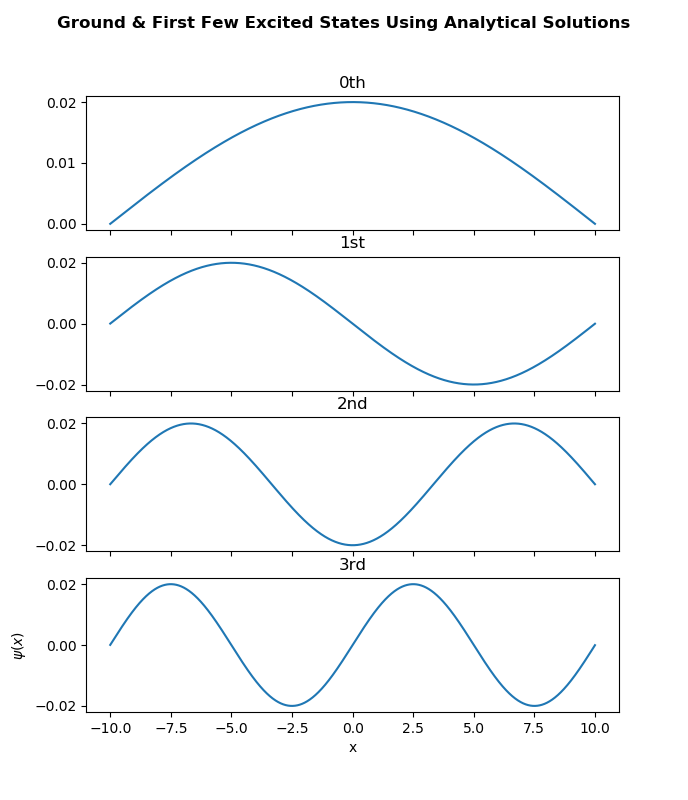
\includegraphics[width=0.5\textwidth]{./particleinabox.png}
	\centering
	\caption{Expected First Few Excited States for a Particle-In-A-Box System}
\end{figure}

\subsection{Three-Point CFD, FFD, BFD Results with no Potential (Particle In A Box)}
\begin{figure}[H]
	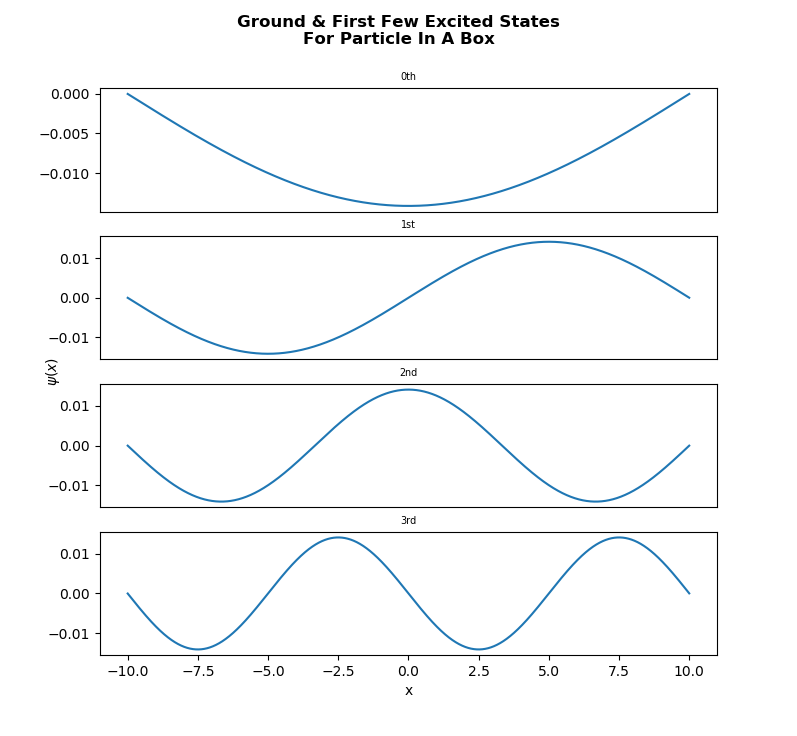
\includegraphics[width=0.75\textwidth]{./particleinaboxCFD.png}
	\centering
	\caption{First Few Excited States of Particle-In-A-Box System Calculated by CFD}
\end{figure}

These results qualitatively mimic the expected ones very closely, with the same numbers of nodes, symmetries, and constant wavelengths. This provides a good indication that this is a good method to use for other, more extravagent, models.

\begin{figure}[H]
	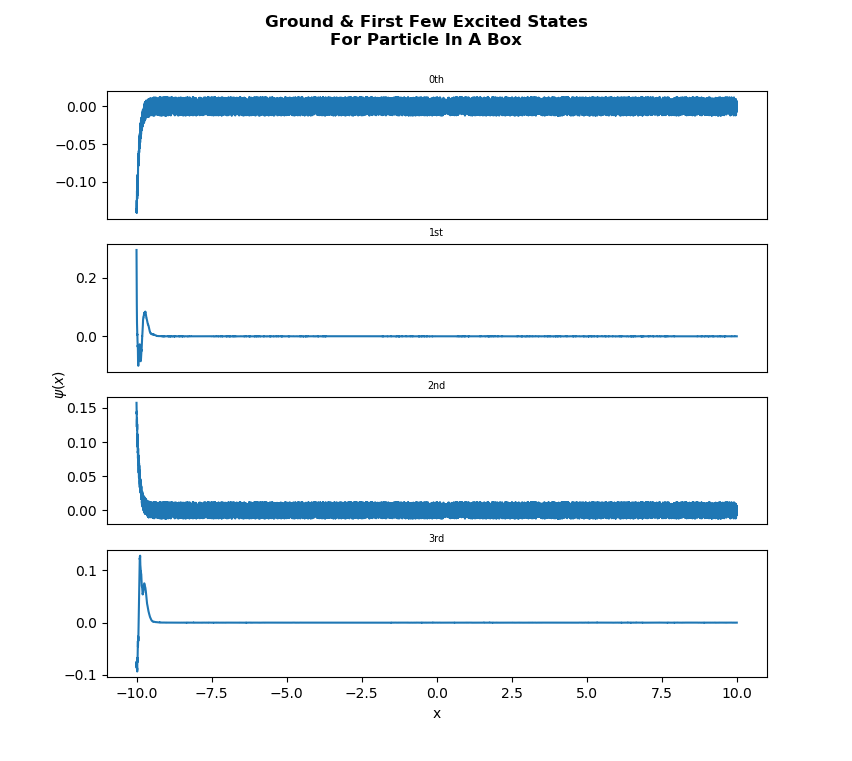
\includegraphics[width=0.75\textwidth]{./particleinaboxFFD.png}
	\centering
	\caption{First Few Excited States of Particle-In-A-Box System Calculated by FFD}
\end{figure}

\begin{figure}[H]
	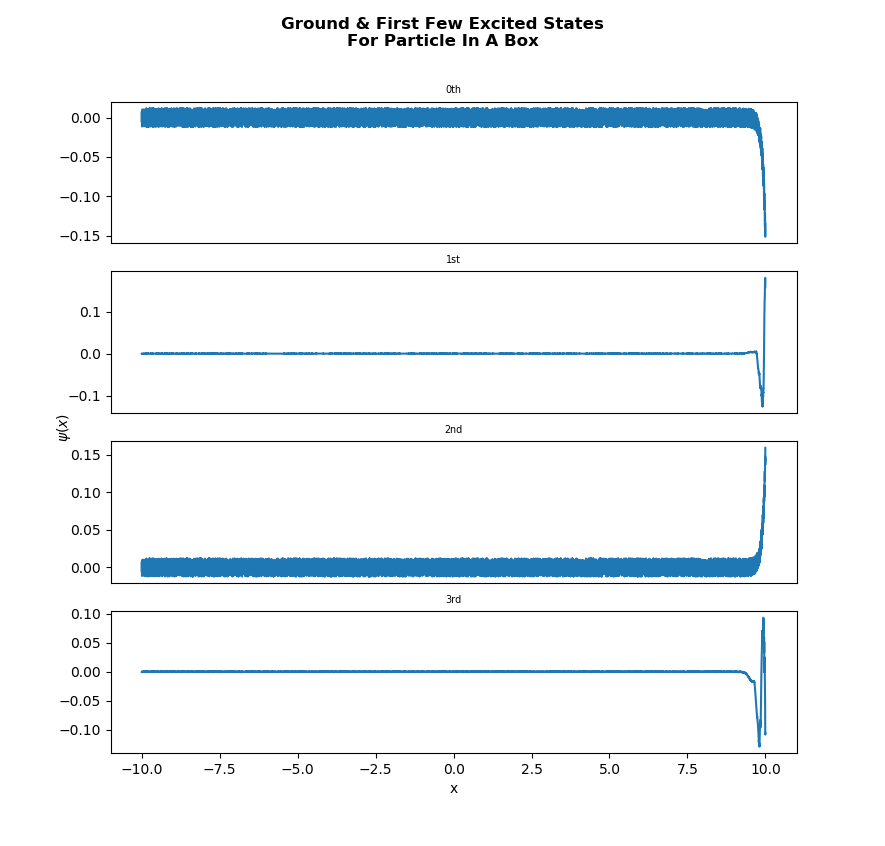
\includegraphics[width=0.75\textwidth]{./particleinaboxBFD.png}
	\centering
	\caption{First Few Excited States of Particle-In-A-Box System Calculated by BFD}
\end{figure}

For both the Forward and Backwards Finite Difference calculations, large stability issues are easily seen. As the same order of finite difference method, and so the same computational expense, was used in all three of these calculations, it is clear that the CFD method is the only one worth developing further. As stated earlier, the CFD method should be accurate to $O(h^{2})$, while the FFD and BFD methods are only accurate to $O(h)$ - this combined with decreased stability resilience resulted in the above calculations, which are not representative of the analytic solutions at all.

\section{Optimisations}

\subsection{Sparse Storage}
The first improvement to the chosen implementation (matrix method) involved moving from storing the Hamiltonian in a standard storage format, in this case a numpy ndarray, to a more suitable data structure; a sparse matrix. 

The motivation for this is that to obtain a solution to a very high accuracy a large number of grid points are needed and, with ndarray storage, the memory needed to store the Hamiltonian scales with the square of the number of grid points - meaning that the maximum possible accuracy is limited by the size of the Hamiltonian that can be held in memory. 

From <ref earlier>, we see that the Hamiltonian is tri-diagonal for our 3 point CFD approach. As a result we know everything about the Hamiltonian if we know its tri-diagonal elements, and so switching to a sparse diagonal storage data structure (scipy's sparse.diags) we can throw away the unneeded zeros and obtain a more efficient Hamiltonian representation that scales linearly with the number of grid points. 

Switching to this data structure expanded the maximum size of Hamiltonian that could be held in memory on my laptop (8GB RAM) from one using 20 thousand grid points to one using over 10 million grid points.

Limitations of this data structure include that more specialised functions are needed to operate on sparse matrices; for example numpy's linalg.eig eigensolver is unable to operate on sparse data. Luckily, scipy's sparse library has a range of equivalent tools designed to replicate the effects of many of numpy's operations for sparse data structure, including several eigensolvers which we now look at as an additional optimisation method.

\subsection{Eigensolver Choice}
As seen in the above section, a sparse storage system allows for more accurate calculations to be performed. There are two main sparse eigensolvers available to use in place of numpy's linalg.eig here; scipy's sparse.linalg.eigs and sparse.linalg.eigsh. These both work similarly, using Arnoldi-based methods for subspace iteration to obtain the eigenpairs, with the difference being that the former uses standard Arnoldi iteration, while the latter uses Lanczos iteration * CITE *. 

Lanczos iteration is a simplification of Arnoldi iteration for the case where the matrix in question is Hermitian; from * cite previous *, we know that a CFD-based Hamiltonian will be real and symmetric - and therefore Hermitian. 

Additional optimisations involving this eigensolver are possible, including the optional parameter `k' which allows the number of desired eigenstates to be specified. By default, the `k' most dominant eigenstates will be returned (dominant implying largest eigenvalue magnitude). 

As we only care about bound states, with eigenvalues below zero, we don't necessarily want the `k' most dominant eigenstates; rather we want the `k' most dominant eigenstates *corresponding to negative eigenvalues*. 

Another optional parameter, `sigma', can be used to achieve this. `sigma' allows a `target' eigenvalue value to be given and, through performing shift-invert preconditioning (* cite my L3? *), the `k' eigenstates closest to that value be returned. 

By passing in a suitably large negative number, we ensure that the returned eigenstates will correspond to the ground state and `k-1'-first excited states. This allows a massive reduction in computational effort needed to obtain particular bound states as, without these, all eigenstates would need to be calculated and then sorted. 

For a model TISE solution using a model with 10k grid points to obtain only the Ground State, and using an estimate for the ground state for the `sigma'/Shift-Invert parameter within 10\% of the real value, the eigsh routine on average took 93.421\% of the time that the eigs routine needed to converge - averaged over 7 trials. 

For the same model and goal; when an estimate that was very far off the real value (around 200 times the real value) was used instead in the Shift-Invert parameter, the eigsh and eigs routines performed very similarly to each other - with eigs being 0.5\% faster averaged over 7 trials.

Using 1 million grid points very similar results were obtained, with eigsh taking 94.753\% as long as eig with the good estimate and 99.832\% as long with a the bad estimate - based on this, it seems the benefit of using eigsh does not scale with Hamiltonian size.

Switching to calculating the Ground state and first 9 excited states, with a 10k grid point model, the benefit of eigsh over eigs for the accurate esetimate appeared to decrease slightly - taking 97.933\% as long, and again for the bad estimate they took very similar times - with eigsh taking 100.263\% as long as eigs.

Additional optimisations involving the `sigma' parameter are described below, which lead to further large reductions in computational expense.

\subsection{FastBOI Improvement}
An additional efficiency improvement that I developed makes use of results from (* cite previous *), where it is seen that the rate of convergence of an eigenstate during subspace iteration is proportional to the magnitude of the corresponding eigenvalue and that eigenstates of of a matrix are also eigenstates of that matrix's inverse (if it exists), with corresponding eigenvalues equal to the reciprocal of the original eigenvalues. 

Combining these it can be seen that if an estimate of an eigenstate's eigenvalue is known, say $\lambda$, then $\lambda I$ can be subtracted from the original matrix to create a new matrix with the same eigenstates, but with eigenvalues equal to the original ones minus $\lambda$. 

As a result, the eigenstate desired will have a `new' eigenvalue of $0$ (or very near, depending on accuracy of the estimate) - thus, if we invert the matrix, the result will have the same eigenvectors but reciprocal eigenvalues, which in the case of the desired eigenstate will be very large and tend towards $\infty$ with increasing accuracy. 

Using the knowledge that the rate of convergence is proportional to eigenvalue magnitude, this shifted and inverted matrix will converge extremely rapidly to the desired eigenstate during subspace iteration, with increased speed if the accuracy to which the original estimate is known is increased.

Based on this result, I developed a `Fast Boosted Optimiser Iteration' method to improve convergence rates for the eigensolver used to find bound states from my Hamiltonian. Another result used in the development of this approach is that a model with fewer grid points than another should still produce relatively correct eigenstates and eigenvalues, simply to a lower accuracy than a model with more grid points. 

Based on these results, the general idea of this approach is to find the ground state eigenvalue for a model with a greatly reduced number of grid points, and then use this as an estimate in the `sigma' parameter of the eigensolver for the model with full number of grid points - greatly increasing the convergence rate for the full model at the cost of having to solve an extra, much smaller, problem. 

Additionally, although only useful for models with a very large number of grid points, this approach can be stacked; a small model can generate an estimate ground state eigenvalue for a medium sized system, which can then generate a better estimate for the full very large system. A flow-chart describing the basic approach is described below, followed by adaptions to allow several `boosting' stages.

Basic FastBOI algorithm:

\begin{figure}[!htb]
	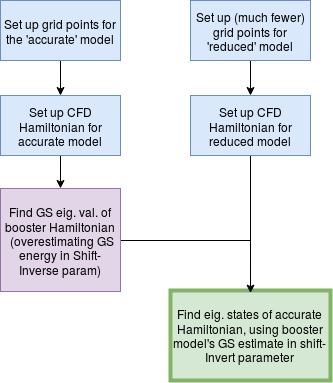
\includegraphics[scale=0.5]{FastBoi}
	\centering
	\caption{Basic FastBOI algorithm}
\end{figure}

Improved (multi-stage) FastBOI algorithm:
\begin{figure}[!htb]
	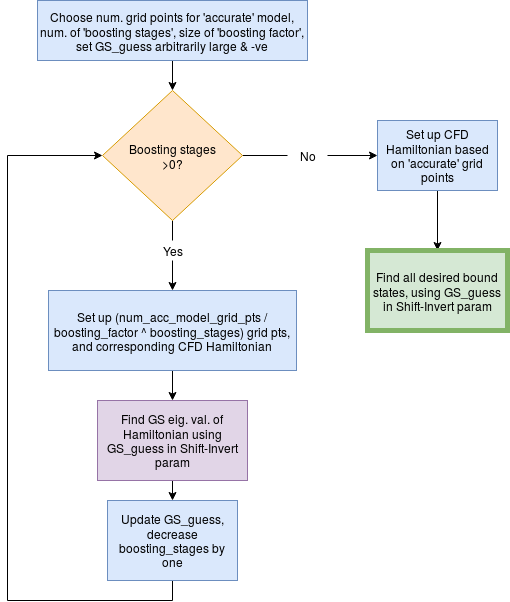
\includegraphics[scale=0.5]{FastBoiImproved}
	\centering
	\caption{Improved (recursive) FastBOI algorithm}
\end{figure}

Using a model with 50 thousand grid points, only seeking the Ground State, and using a very large negative number (around $10^{3}$x the real energy) as the baseline estimate - using the FastBOI algorithm with a boosting factor of 100 and a single boosting stage was 90.948 times faster than not using it, jumping to 107.928 times faster when the boosting factor was increased to 1000. 

Using the same comparison, but with a 500 thousand grid point model, the FastBOI algorithm with 1 boosting stage and a boosting factor of 100 was 58.914 times faster than without, with 1 boosting stage and a boosting factor of 1000 it was 77.749 times faster, and with 2 boosting stages and a boosting factor of 100 it was 87.1 times faster. 

It was noticed that the time to solve the model without using the FastBOI algorithm scaled linearly with model size - and so for the following, larger, models estimates were used for the comparisons as each calculation woud otherwise take several hours. With this assumption; for a model with 5 million grid points and only seeking the ground state, the FastBOI algorithm with 1 boosting stage and a boosting factor of 1000 was about 89 times faster, with 2 boosting stages and a boosting factor of 250 it was about 96 times faster, with 3 boosting stages and a boosting factor of 40 it was about 93 times faster, and with 4 boosting stages and a boosting factor of 10 it was about 85 times faster.

Larger models were uable to fit into RAM on my laptop, and so could not be tested.


%definition of variables:
%\begin{itemize}
%
%	\item[-]{\textbf{x_full:} The grid points for the full accuracy model}
%	\item[-]{\textbf{x_red:} The grid points for the reduced accuracy model, it will have the same start- and end-points as x_full}
%	\item[-]{\textbf{boosting_factor:} The relative size of x_full to x_red}
%
%\end{itemize}

%\begin{lstlisting}
%function basic_fastboi(x_full, boosting_factor){
%	start, end, size = x_full[0], x_full[last], SIZE(x_full);
%	inc = (end - start) / (size / boosting_factor);
%	x_red = ARRAY();
%
%	for i = 0..(size / boosting_factor){
%		x_red[i] = start + i*inc;
%	}
%
%	H_red = generate_hamiltonian(x_red); 
%	est_GS_eigval, est_GS_eigvec = eigensolver(H_red, sigma = -B);
%	
%	/* where B is some arbitrarily large number such that B
%	   is definitely less than the real GS eigenvalue.
%	   Note: matching the output of ARPACK and LAPACK eigensolver outputs,
%	   only est_GS_eigval needed
%	*/ 
%	
%	H_full = generate_hamiltonian(x_full);
%	acc_GS_eigval, acc_GS_eigvec = eigensolver(H_full, sigma = est_GS_eigval);
%	
%	return (acc_GS_eigval, acc_GS_eigvec);
%}
%\end{lstlisting}
%
%As mentioned, this `boosted optimiser' approach can be stacked iteratively allowing a more accurate estimate to be generated for the full accuracy model, at less than the cost of solving a medium size model with an arbitrarily large negative number that would otherwise be needed. The adaption to the above algorthm to allow several boosting stages is described as follows, using a recursive approach;
%
%\begin{lstlisting}
%function fastboi(x_full, boosting_factor, num_boosts, estimate=-B){
%	start, end, size = x_full[0], x_full[last], SIZE(x_full);
%	inc = (end - start) / (size / (boosting_factor^num_boosts));
%	x_red = ARRAY();
%
%	for i = 0..(size / boosting_factor){
%		x_red[i] = start + i*inc;
%	}
%
%	H_red = generate_hamiltonian(x_red); 
%	est_GS_eigval, est_GS_eigvec = eigensolver(H_red, sigma=estimate);
%	
%	if (num_boosts > 0){
%		return fastboi(x_full, boosting_factor, num_boosts-1, est_GS_eigval);
%	}
%	else{
%		H_full = generate_hamiltonian(x_full);
%		acc_GS_eigval, acc_GS_eigvec = eigensolver(H_full, sigma = est_GS_eigval);
%		return (acc_GS_eigval, acc_GS_eigvec);
%	}
%}
%\end{lstlisting}
%
\subsection{Pre-Trained Predictive Model Improvement}

An alternative to the Boosted Optimiser Iteration method, suitable for other use cases, is to find estimates to the Ground State energy for many differently shaped potentials and train a predictive model to generate an estimate to use for the Shift-Invert parameter of the eigensolver based on the shape of the potential being used. To investigate this approach I used reduced models with 1000 grid points, and generated 1000 different potentials. 

For each model I then found the ground state eigenvalue, using a massively negative estimate in the Shift-Invert parameter, and then recorded the ground state value along with statistics to describe the potential used in that model; such as mean, median, skew, standard deviation, kurtosis. 

Several machine learning models, including a 3-hidden-layer neural network and a boosted random forest, were trained on a randomly selected 85\% of the data. After feature selection and hyperparameter tuning, the models ranged from 97.3\% (simple linear regression) to 99.996\% (neural network) accurate on the unseen 15\% of the data (measured using Mean Average Error).
Once trained, these predictive models can be saved for future usage - allowing for a near-immediate Ground State estimate in the future as opposed to having to solve one or more reduced models every time. 

Using a prediction from the neural network model in the Shift-Invert parameter when solving a 10k grid point model gave around a 400x speedup compared to using a large negative guess - including the time taken to generate statistics about the potential and feed them into the neural network. 

Limitations of this approach include that, unless similar calculations are going to be performed often, the time taken to generate the synthetic data and train the predictive model is much greater than the cost of not using a good ground state estimate, and also that this approach can't `stack' like the Boosted Optimiser Iteration approach - limiting the speedup benefit for very high-precision models. 

Advantages of it are that, once trained, there is very little extra work or computational effort needed to allow the speedup, and also over time the higher-accuracy ground state energies that are calculated can be saved and the predictive model retrained using them.


%----------------------------------------------------------------------------------------
